\section{Comparaison avec la photo en contraste
élevé}\label{comparaison-avec-la-photo-en-contraste-uxe9levuxe9}

\begin{figure}[htbp]
\centering
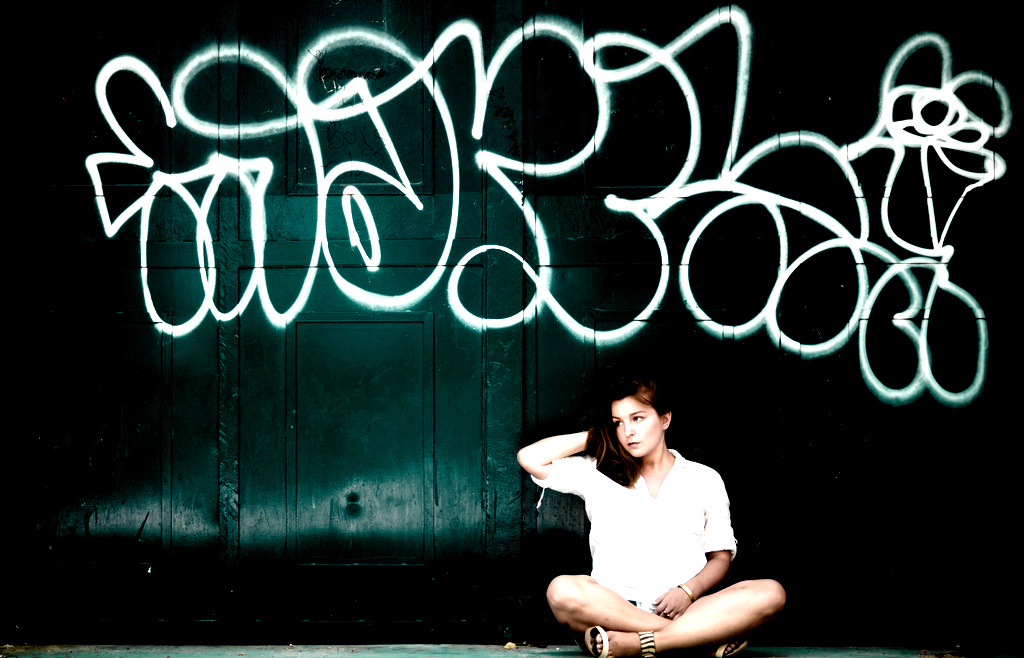
\includegraphics{../../photos/contraste.jpg}
\caption{Photo contraste}
\end{figure}

\begin{table}[htbp]
\centering
\begin{tabular}{llr}
\bfseries Formes (\%) &
\bfseries Bhattacharyya (\%)%
\DTLforeach*[\DTLiseq{\fichier}{photos/contraste.jpg}]{valeurs}{%
\fichier=Fichier, \formes=Formes,\bhatta=Bhattacharyya, \hue=Hue, \saturation=Saturation, \value=Value}{%
\\
\formes & \bhatta}
\end{tabular}
\end{table}

La comparaison de la photo originale avec la photo en
contraste élevée nous donne comme résultat que les deux /photos se
ressemblent au niveau de leurs formes mais pas suffisamment d'un point
de vue colorimétrique. \\
Cela s'explique par le fait qu'augmenter les contrastes d'une photo change ses
couleurs et très peu sa forme (on a relevé seulement $28 \%$ de différence par
comparaison après l'application d'un filtre de Sobel contre $35 \%$ de différence
avec la distance de Bhattacharyya).
